\documentclass[10pt]{article}
\usepackage[utf8]{inputenc}
\usepackage{fullpage}
\usepackage[backend = bibtex]{biblatex}
\addbibresource{sample.bib}
\usepackage[english]{babel}
\usepackage{tabularx}
\usepackage{amsmath,amssymb}
\usepackage{graphicx}
\usepackage{grffile}
\usepackage{multicol}
\newcolumntype{C}{>{\centering\arraybackslash}X}
\begin{document}
	\newpage
	\begin{center}
		\Huge \textbf{Stroke Recognition from Characters}
		\\[180pt]
		\Large Interim Report of B.Tech IT $5^{th}$ Semester Mini-Project
		\\[100pt]
		\Large Supervised By\\Prof. Sudip Sanyal
		\\[100pt]
		\underline{Group Members}
		\\[20pt]
		Kaustubh Shamshery \hspace{40pt} Pratik Mangalore\\Prateek Agarwal \hspace{60pt}Sulyab Thottungal     
	\end{center}
	\large
	\newpage
	\begin{center}
		\Huge \textbf{Candidate's Declaration}
		\\[120pt]
		\Large
		We hereby declare that the project report titled
		
		``Stroke Recognition from Characters" submitted by us to
		
		Indian Institute Of Information Technology, Allahabad,
		
		in partial fulfillment of the $5^{th}$ semester Mini-Project work,
		
		is a record of bonafide project work, 
		
		under the supervision of Prof. Sudip Sanyal.
		\\[100pt]
		\underline{Group Members}
		\\[50pt]
		Kaustubh Shamshery \hspace{40pt} Pratik Mangalore\\[50pt] Prateek Agarwal \hspace{60pt}Sulyab Thottungal
	\end{center}
	\newpage
	\begin{center}
		\Huge \textbf{Supervisor's Certificate}
		\\[100pt]
		\Large
		This is to certify that the project report entitled
		
		``Stroke Recognition from Characters"	
		
		submitted to Department of Information Technology,
		
		Indian Institute of Information	Technology, Allahabad
		
		in partial fulfillment of the $5^{th}$ semester Mini-Project work,
		
		is a record of bonafide work carried out by :
		\\[30pt]
		1. Kaustubh Shamshery – IIT2014147
		
		2. Pratik Mangalore – IIT2014112
		
		3. Prateek Agarwal – IIT2014068
		
		4. Sulyab Thottungal – IIT2014125
		\\[30pt]
		under my supervision and guidance.
		
		No part of this report has been submitted elsewhere for any other purpose.
		\\[100pt]
		\flushright
		\textbf{Prof. Sudip Sanyal}
		
		Dean (Research and Development)
		
		Department of Information Technology
		
		Indian Institute of Information Technology
		
		Allahabad 211 012, India
	\end{center}
	\newpage
	\hrulefill
	\tableofcontents
	\hrulefill
	\newpage
	\large
	\section{Abstract}
		\hrulefill
		\paragraph{Background :}
		Probabilistic Latent Semantic Analyis is a statistical technique used for the analysis of co-occurence data. In effect, one can derive a low-dimensional representation of the observed variables in terms of their affinity to certain hidden variables. We apply the above technique on a dataset consisting of images of characters in order to derive strokes which can generate the complete alphabet. The strokes here are the hidden variables which are a low-dimensional representation of the observed variables - pixels, in this case.
		\paragraph{Purpose of Research :}
		The human brain learns by recognizing patterns in the data that it is fed. Similarly, it is seen that we recognize the characters in an alphabet based on the different kinds of strokes they have. Here, a stroke is a unique formation of pixels, which co-occur regularly in the characters and do not belong to other strokes. We are using the PLSA technique on the character images so as to find out these strokes in a manner not very unlike how we humans learn.
		\paragraph{Methods Used :}
		We are primarly using the following methods to generate the strokes :- \\
		1) Probabilistic Latent Semantic Analysis\\2) Expectation Maximization Algorithm (As an internal step in PLSA)	
		\paragraph{Current Result :}
		By applying the PLSA technique (using EM) on the dataset, we have been able to obtain strokes which can be combined in order to recreate the characters in a given alphabet.
		\paragraph{Conclusion :}
		We conclude that the PLSA algorithm which until now is usually used in the domain of NLP can be modified so that it can be applied to images with greater levels of accuracy.
	\newpage
	\section{Introduction}
		\hrulefill
		\subsection{Overview}
			Recognition of printed characters and handwriting is a subfield of prime importance in computer vision and artificial intelligence domains. Digitalization of information for safe storage and efficient manipulation has become a necessity in this era of information explosion.\\\\
			Character recognition has been implemented very efficiently using many techniques in the past few decades. However, in this project, we explore a new method - identifying the strokes required to generate an entire alphabet. Here, strokes mean the basic curves which add up to produce whole letters. 
			
		\subsection{Motivation}
			Identification of strokes is important as it gives and takes from how the human brain recognizes objects. The human brain uses information of orientation and spatial relations to identify objects. \cite{dicarlo}\\\\
			We propound the idea that the identification of strokes using PLSA on the characters' images is analogous to the manner in which our brain learns and recollects information. Using this method to identify characters might, in turn, provide more insight into the intricate ways of brain functioning.
		\subsection{Scope}
			The latent variables generated in this algorithm are the strokes present in the alphabet itself, and they are learnt by the algorithm in an unsupervised fashion. This makes the algorithm script-independent. Also, the EM algorithm converges faster than the backpropagation algorithm  which is used in neural nets, which is a popular alternative for character recognition.
		\subsection{Problem Definitions and Objectives}
			Stroke Definition :-\\We define a stroke as a unique co-occurence of pixels which exhibit a specific spatial orientation.\\\\ 
			Objective :-\\Given a dataset consisting of grayscale images of characters in a script, the strokes that completely generate the script are to be identified using unsupervised learning approach.
			The probability that a particular pixel of a particular character is black, can be expressed using the probability distribution of strokes as\\
			\begin{equation}
			P\,(x_i|c_j)=\sum_{k\in S} P\,(s_k|c_j)P\,(x_i|s_k)
			\end{equation}
			where $x_{i}$ is the event that the $i^{th}$ pixel is black, $c_{j}$ is the $j^{th}$ letter in the script, $s_{k}$ is the $k^{th}$ stroke that has been identified, and S is the set of all strokes.\\\\
			The above expression contains latent (hidden) variables in its RHS, and hence cannot be determined directly. Hence, we adopted the PLSA (Probabilistic latent semantic analysis) model, which is a statistical technique for automated document indexing. In PLSA, the probability of each variable is modelled as expressions involving conditionally independent multinomial distributions.
		\subsection{Organization of the Project}  
		    For effecient collaboration, we used Google Drive and a private GitHub repository.\\\\
		    Each one of us had our own working dataset on which ran the algorithm separately, each time changing the definitons or number of sample/stroke. 
	\newpage
	\section{Literature Survey}
	\hrulefill
	\subsection{Background and Related Work}
		\begin{tabularx}{15cm}{| l | c | C | C |}
			\hline 
			Sr.No & Author/Website/Book & Paper Title & Referenced For \\
			\hline
			1 & Thomas Hoffman &  “Probabilistic latent semantic analysis,” in Proceedings of the fifteenth conference on uncertainty in artificial intelligence,  1999, pp. 289-296. & Theory related to the PLSA algorithm and how topic categorization relates to dividing characters into strokes. \\
			\hline 
			2 & Thomas Hoffman & “Unsupervised learning by probabilistic latent semantic analysis,” Machine learning, vol. 42, iss. 1-2, pp. 177-196, 2001 & How the EM algorithm is used in PLSA in order to maximize the likelihood of presence of stroke in a character such that a pixel exists in it.\\
			\hline 
			3 & DataEra.org & Notes on EM and pLSA”& For referring the mathematical steps used in the EM algorithm.\\
			\hline 				
		\end{tabularx}
	\subsection{Concluding Remarks on the basis of Literature Survey}
		After completing the research survey it was found that, the PLSA algorithm could in fact be used on images with definite success. We know this because the definitions in the case when PLSA is applied on document and words are similar to the definitions when PLSA is applied on images.
		
	\newpage
	\section{Plan Of Work}
	\hrulefill
	\subsection{Proposed Approach}
		\large We divided our work into the following parts :-
		\subsubsection{Preprocessing} 
			\begin{itemize}
				\item 
				At the start all the sample images were of different sizes. Therefore, we decided to resize them into a square image of side length 40. Not only would this make the image uniform, but it would also reduce the running time of the algorithm.
				\item
				We also generated the Term Document Matrix \cite{hoff1}, which will be used by the PLSA algorithm. The 2517 rows in the Term Document matrix represent the images in the dataset whereas the 1600 columns represent the grayscale value of each pixel.
			\end{itemize}
		\subsubsection{Definitions}
			Firstly, lets define a few entities. 
			\begin{itemize}
				\item 
				Let N be the number of image samples (this is analogous to number of documents) which we have currently taken to be 2517.
				\item
				Let M be the number of pixels in our images (this is analogous to number of words in our vocabulary) which is clearly 1600 (40x40).
				\item
				$w_j$ refers to the $j^{th}$ pixel (i.e, 0 to 1599) being black, and $d_i$ refers to the $i^{th}$
				image (i.e, 1 to 2517)
				\item 
				The below equation gives the log-likelihood function which we want to maximize in the general EM algorithm
				\begin{equation} 
				L(\theta) = \log P(y|\theta) = \log \sum_{z} P({y,z}|\theta)
				\end{equation}
				The following equation \cite{hoff2} shows the log-likelihood function obtained from the PLSA model
				\begin{equation}
					log P(d,w) = \sum_{i=1}^{N}\sum_{j=0}^{M-1}n(d_i,w_j)log P(d_i,w_j)
				\end{equation}
				\item
				In the log-likelihood function (3), we find a log structure with latent variable that is very similar to the log-likelihood function (2) of a general EM problem. Hence, we can apply EM algorithm to the PLSA model to maximize the log-likelihood.
			\end{itemize}
		\subsubsection{Applying EM algorithm on the PLSA model}
			Few more definitions for the PLSA model \cite{hoff1} :-
			\begin{itemize}
				\item 
				$P(z_k|d_i,w_j)$ is the posterior probability that $k^{th}$ stroke exists given that $i^{th}$ image is considered and $j^{th}$ pixel is black.
				\item
				$P(w_j|z_k)$ is the probability that the $j^{th}$ pixel is black and exists in the $k^{th}$ stroke.
				\item
				$P(z_k|d_i)$ is the probability that the $k^{th}$ stroke exists in $i^{th}$ image.
			\end{itemize}
			The Expectation-Maximization \cite{dataera} algorithm, applied to PLSA model is as follows :
			\subparagraph{Initialization :}
				Initialize the parameters $P(z|d)$ and $P(w|z)$ randomly
			\subparagraph{Repeat until convergence :}
			\begin{itemize}
				\item
				E-STEP :- 
				\[ P\,(z_k|d_i,w_j) = \dfrac{P\,(w_j|z_k)P\,(z_k|d_i)}{\sum_{l=1}^{K}P\,(w_j|z_l)P\,(z_l|d_i)} \]
				\item
				M-STEP :-
				\[ P\,(w_j|z_k) = \dfrac{\sum_{i=1}^{N}n\,(d_i,w_j)P\,(z_k|d_i,w_j)}{\sum_{m=1}^{M}\sum_{i=1}^{N}n\,(d_i|w_m)P\,(z_k|d_i,w_m)} \]
				\[ P\,(z_k|d_i) = \dfrac{\sum_{i=1}^{N}n\,(d_i,w_j)P\,(z_k|d_i,w_j)}{n(d_i)} \]
			\end{itemize}	 
	\subsection{Dataset Description}
		The original dataset contained two groups of characters which represent the consonants and the vowels of the Tibetan script. The first group had 211 characters, each having 20-50 samples. The original dataset contained images of non-uniform dimensions. We first resized the images to 40x40 for uniform sizing and reducing the running time of the program.
		
	\subsection{Software Requirements}
		\subparagraph{Hardware}
			\begin{itemize}
				\item 
				Python (including  numpy, matplotlib, os, PIL, datetime packages) \cite{pytho}
				\item
				Git and GitHub
			\end{itemize}
	\subsection{Activity Time chart}
		The task was divided as follows:-
		\begin{center}
			\begin{tabular} {|| c | c || }				
				\hline 
				\textbf{Task} & \textbf{Expected time} \\
				\hline
				Literature Survey & 2 weeks \\
				\hline 
				Problem Identification & 1 week \\
				\hline 
				Project Implementation & 1 week \\
				\hline 
				
			\end{tabular}
		\end{center}	
	\newpage
	\section{Results and Analysis}
		\hrulefill
		\subsection{Results :}
			\begin{itemize}
				\item
				We ran the EM algorithm on our PLSA model by passing the number of strokes as a parameter. Different stroke patterns were obtained for different input.
				\item
				We observed that the stroke patterns generated depended on number of strokes and size of the dataset used.
				\item
				$P\,(w_j|z_k)$ and $P\,(z_k|d_i)$ converged after about 100 iterations.
				The breaking condition here is if the likelihood changes by less than a factor of $10^{-6}$.
			\end{itemize}
			\begin{center}
				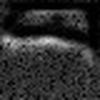
\includegraphics{stro0.jpg}
				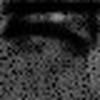
\includegraphics{stro1.jpg}
				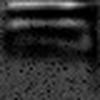
\includegraphics{stro2.jpg}
				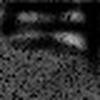
\includegraphics{stro3.jpg} \\
				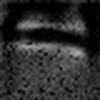
\includegraphics{stro4.jpg}
				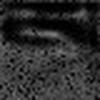
\includegraphics{stro5.jpg}
				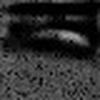
\includegraphics{stro6.jpg}
				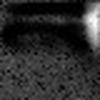
\includegraphics{stro7.jpg} \\
				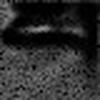
\includegraphics{stro8.jpg}
				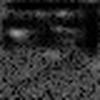
\includegraphics{stro9.jpg}
			\end{center}
		\subsection{Analysis :}
			\begin{itemize}
				\item 
				Depending on the size of dataset we used to train the algorithm, the time taken for generating the strokes ranged from 1-5 hrs. The strokes generated were much more accurate and clear when the PLSA model ran on a larger dataset.
				\item
				The time complexity of our program is O(NMK) which equates to about $10^{9}$ instructions of python code to execute. Here, N stands for the number of images, M stands for the size of each image, and K stands for number of strokes.
			\end{itemize}
	\newpage
	\section{Conclusion and Future Scope}
		\hrulefill \\\\
		Analysing the work done so far, we conclude that carrying out stroke recognition from images using PLSA technique is highly effective.\\\\The following tasks are to be done next :
		\begin{itemize}
			\item 
			Decompose the ‘strokes’ obtained into simpler, basic strokes without changing the unsupervised nature of the algorithm
			\item
			Optimize the algorithm and reduce its running time
			\item
			Devise a method to extract the minimum number of strokes required to completely and accurately generate a given script, while taking care of overfitting issues
			\item
			Refine the obtained stroke images by reducing noise
		\end{itemize}
	\newpage
	\printbibliography
	\newpage
	\section{Suggestions And Remarks :}
		\hrulefill\\
		\Large Please write down your suggestions and remarks if any:	
\end{document}